\chapter{Algoritmos}
\label{sec:algoritmos}
En esta sección se va a comentar los distintos algoritmos que han sido usados para la resolución del problema que se aborda en este trabajo.\\
A la hora de seleccionar un algoritmo para resolver un problema, no se puede elegir el algoritmo $X$ por ser 'el mejor'. Para apoyar esta idea, los investigadores David Wolpert y William Macready publicaron un artículo donde establecen el teorema \textbf{\textit{No-Free-Lunch}} (NFL).\\
\textbf{NFL} afirma que el \textbf{rendimiento medio} por cada par de algoritmos aplicados a todos los posibles problemas es idéntico.Partiendo de esta idea, se han seleccionado una serie de algoritmos que van a ser usados y cuyo rendimiento va a ser analizado en secciones siguientes. \\
\linebreak
Esta sección está enfocada en introducir los algoritmos seleccionados para facilitar la comprensión de los resultados.
\section{Árboles de decisión}
\label{alg:dec_tree}
Los árboles de decisión son una técnica de aprendizaje supervisado que se puede usar para clasificación y regresión. Esta técnica hace uso de \textbf{reglas} del tipo \textit{si variable cumple condición entonces } inferidas a partir de los datos. \\
Este tipo de técnicas son fáciles de representar usando una representación en árbol:
\begin{itemize}
	 \item Los nodos internos del árbol representan las características del conjunto de datos.
	 \item Las ramas se usan para representar las \textbf{decisiones} tomadas por el algoritmo.
	 \item Los nodos hojas se utilizan para representar la salida.
\end{itemize}
El algoritmo básico que usan los árboles de decisión consta de los siguientes pasos:
\begin{enumerate}[1º]
	  \item Se comienza en el nodo raíz que contiene el conjunto de datos completo.
	  \item Elegir una variable del dataset utilizando una \textbf{heurística}.
	  \item Dividir el nodo raíz en distintos nodos para contener todos los posibles valores de la característica seleccionada en el paso anterior.
	  \item Repetir el proceso anterior hasta que no se pueda dividir en más conjuntos.
\end{enumerate}
El uso de una buena heurística a la hora de elegir la variable es clave a la hora de generar una buena división del conjunto de datos, provocando así un modelo con una buena capacidad de predicción. Algunas de las heurísticas que más se usan son:
\begin{itemize}
	\item \textbf{Indice GINI}: Los árboles construidos con este método se conocen como \textbf{CART}
	\item \textbf{Ganancia de información:} Los árboles construidos con este método se conocen como \textbf{ID3}
\end{itemize}
Los árboles de decisión ofrecen ciertas ventajas:
\begin{enumerate}
	\item Son modelos fáciles de interpretar y pueden ser visualizados.
	\item Son capaces de trabajar con variables categóricas y numéricas.
	\item introducir alguna ventaja más
\end{enumerate}
Sin embargo, también presentan ciertas desventajas:
\begin{enumerate}
	\item Modelos que tienden al sobre-aprendizaje.
	\item No soportan valores perdidos.
	\item No trabajan bien con conjuntos de datos des-balanceados.
\end{enumerate}
\section{Random Forest}
\label{alg:rf}
Random Forest es un modelo combinado de aprendizaje que puede usarse para clasificación y/o regresión. Random Forest consiste en un conjunto de árboles de decisión que operan juntos. Una vez que cada árbol dentro del Random Forest realiza una predicción, se escoge la predicción con más votos. \\ Se ha escogido este modelo ya que como se comprobó en la sección \textbf{\ref{alg:dec_tree}-\nameref{alg:dec_tree}}, los árboles de decisión dieron buenos resultados
\linebreak
Para que Random Forest funciona bien, hay que asegurar que los distintos árboles que lo forman tengan una baja \textbf{correlación} entre ellos. Esto quiere decir que los árboles tienen que diferir y proporcionar predicciones distintas, de esta manera, si hay un conjunto de árboles que da una predicción malas, puede haber otro conjunto que vaya en la dirección correcta. \\
\linebreak
Los Árboles de Decisión son modelos que son muy sensibles a los datos con los que se ha entrenado, por lo que cualquier cambio en los datos de entrenamiento puede hacer que cambie una predicción. Random Forest hace uso de esta peculiaridad de los árboles de decisión.
En el momento de entrenar los distintos árboles, en vez de usar subconjuntos del conjunto de entrenamiento se usan $N$ conjuntos del mismo tamaño que el conjunto de entrenamiento obtenidos usando un \textbf{muestreo con reemplazo}. Una vez que se tienen los distintos conjuntos, se entrena cada conjunto con un árbol. Este proceso se conoce como \textbf{bagging}.\\
\linebreak
Una peculiaridad más que tiene Random Forest es la forma con la que los árboles seleccionan la variable que van a usar para dividir el conjunto de datos. Estos no eligen la variable en función de un criterio concreto, si no que eligen la variable usando un conjunto aleatorio de las características. Esto fuerza a que los árboles sean mas diferentes entre ellos, bajando la correlación entre los árboles que forman el modelo.
\section{KNN}
\label{alg:knn}
KNN (\textit{K Nearest Neighbors}) es un algoritmo supervisado basado en instancias. Este algoritmo no aprende un modelo si no que almacena todas las muestras de entrenamiento y cuando hay que predecir una nueva ejemplo, el algoritmo usa las muestras almacenadas calculando la distancia a cada muestra y obteniendo los K vecinos más cercanos y usando las valores reales de los vecinos seleccionados, asigna una predicción al ejemplo a predecir, generalmente asignando aquella clase con más "votos".\\
\linebreak
Para medir la distancia entre dos muestras, KNN puede usar una gran cantidad métricas, las más comunes son:
\begin{itemize}
	\item \textbf{Distancia euclidiana:} Definida como $\sqrt{\sum(x_1 - x_2)^2}$
	\item \textbf{Distancia Manhattan:} Definida como $\sum|x_1 - x_2|$
	\item \textbf{Distancia Minkowski:} Definida como $(\sum|x_1 - x_2|^p)^{\frac{1}{p}}$, siendo P un entero positivo
\end{itemize}
La implementación del algoritmo KNN de \textit{scikit-learn} usa por defecto la distancia \textbf{Minkowski}. Esta tiene la peculiaridad de que cambiando el parámetro $p$ puede usarse la distancia euclidiana ($p=2$) o la distancia Manhattan ($p=1$)
\section{SVM}
\label{alg:svm}
Maquina de soporte de vectores (Support Vector Machines) es un modelo de aprendizaje supervisado cuyo objetivo es encontrar un hiper-plano dentro de un espacio de $N$ dimensiones ($N$ es el número de características del conjunto de datos) que clasifique las muestras de dentro del espacio en distintas clases. Originalmente, se diseñó para clasificación binaria, pero en la actualidad este algoritmo se ha adaptado para regresión, clasificación multi-clase y multi-etiqueta\\
\linebreak
Pueden existir muchos hiper-planos que separen los puntos del espacios en distintas clases. El objetivo de SVM es encontrar aquel hiper-plano con mayor \textbf{margen} (distancia entre puntos de distintas clases), ya que incrementa la posibilidad de clasificar correctamente muestras que no se han usado en entrenamiento al disponer de un margen mayor de error. Los vectores soporte son aquellas observaciones del conjunto de datos que definen el hiper-plano. Idealmente, estas o\\
\begin{figure}[H]
	\centering
	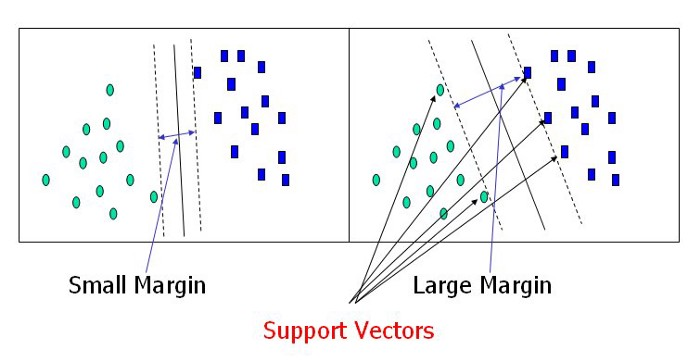
\includegraphics[scale=0.5]{svm}
	\caption{Ejemplo de SVM en dos dimensiones}
	\label{fig:svm}
\end{figure}
\section{XGBoost}
\label{alg:xgb}
Extreme Gradient Boosting es un método de aprendizaje combinado basado en árboles de decisión.\\
A diferencia de Random Forest (que también es un método combinado basado en árboles de decisión), XGBoost hace uso de técnicas de \textit{Gradient Boosting} frente a Random Forest que hace uso de \textit{Bagging} para entrenar los modelos que lo forman. (\ref{sec:rf}-\nameref{sec:rf}).\\
\linebreak
\textit{Boosting} se basa en la unión de varios modelos débiles para formar un modelo que en conjunto. Estos modelos débiles se van entrenando de forma iterativa, adaptando los parámetros del modelo en cada iteración, teniendo en cuenta que estos modelos no deben aumentar en complejidad y deben mantener un rendimiento mínimo (idealmente, mejor que un clasificador aleatorio).\\
\linebreak
\textit{Grandient Boosting} es un caso especial de \textit{Boosting} en el que se hace uso del algoritmo \textbf{Gradiente Descendente} para minimizar los errores de los modelos simples.\\
\linebreak
Finalmente, XGBoost funciona añadiendo secuencialmente Árboles de Decisión, de tal manera que cada árbol reduzca el error de los previos aprendiendo de los errores que han cometido los árboles anteriores.
\section{Perceptrón multi-capa}
\label{alg:mlp}
El Perceptrón Multicapa es un modelo de aprendizaje supervisado basada en red neuronales artificiales y haciendo uso del algoritmo \textbf{Perceptrón}.\\
\linebreak
El Perceptrón es un algoritmo de aprendizaje supervisado para clasificación binaria. Es un clasificador linear que funciona iterando sobre cada muestra del conjunto de datos hasta calcular un hiper-plano que separe el conjunto de datos. Los pasos de este algoritmo son:
\begin{enumerate}
	\item Establecer un plano inicial (generalmente de manera aleatoria ).
	\item Por cada muestra del conjunto de datos, si la muestra está mal clasificada, se modifican los pesos que definen el hiper-plano para clasificar correctamente esa muestra.
	\item El paso anterior se repite hasta que todas las muestras estén bien clasificadas ó no se haya hecho ninguna modificación. Por lo general, también se añade un número máximo de iteraciones que se van a realizar.
\end{enumerate}
Este algoritmo tiene una limitación muy fuerte: No puede resolver problemas no lineales (incluso funciones sencillas como la \textit{XOR}). \\
\linebreak
Para afrontar este problema, se propuso el usar una combinación de perceptrones siguiendo una estructura de red neuronal, consiguiendo así un modelo capaz de resolver problemas no lineales. Estas redes neuronales tienen al menos 3 capas:
\begin{itemize}
	\item Capa de entrada: Está formada por las primeras neuronas que forman la red y se encargan de introducir los datos a la red.
	\item Capa/s oculta: Son las capas de la zona media de la red y son las encargadas del procesamiento de los datos para formar el modelo.
	\item Capa de salida: Dan el valor de salida del modelo.
\end{itemize}
\begin{figure}[H]
	\centering
	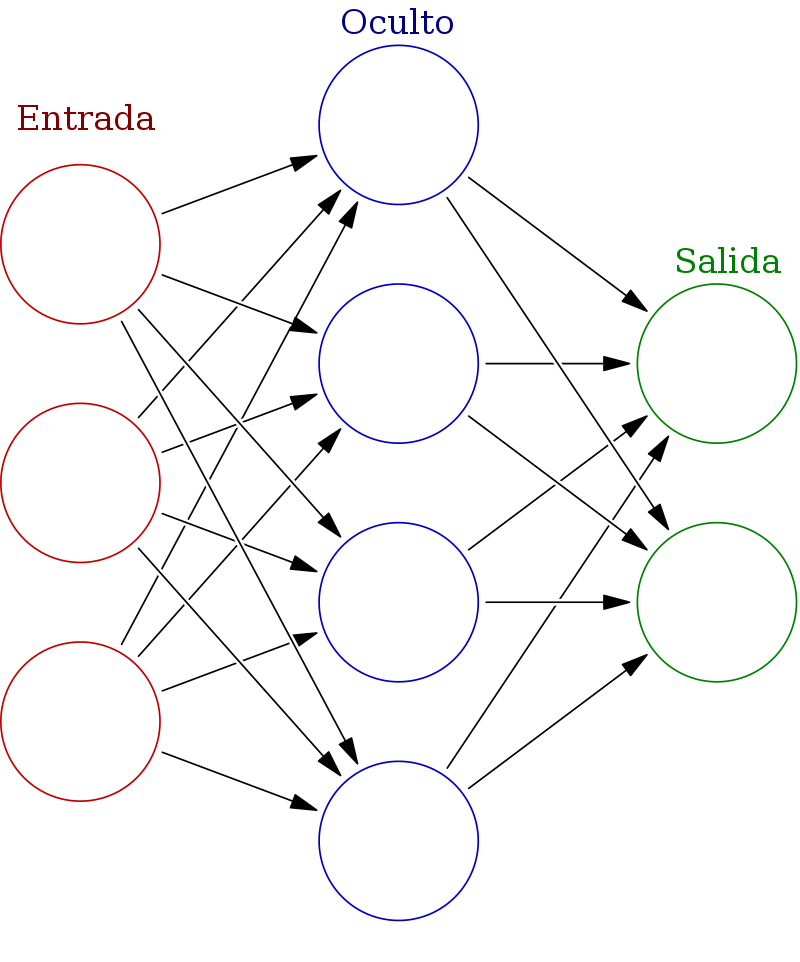
\includegraphics[scale=0.3]{rnn}
	\caption{Ejemplo de Red Neuronal con 1 capa oculta}
	\label{fig:rnn}
\end{figure}
Un elemento fundamental de las Redes Neuronales es el algoritmo de \textit{back-propagation}. Este algoritmo usa el error obtenido en las capas de salida y este era propagado hacia cada neurona anterior (de ahí el nombre de \textit{back-propagation}), ajustando así el peso calculado por cada neurona en función del comportamiento del modelo en la iteración anterior.
\section{Conjuntos de validación}
\label{sec:validation}
Finalmente en esta sección, se va a explicar que metodología se ha seguido para determinar el la capacidad de predicción del modelo seleccionado, ya que no basta con definir un conjunto de entrenamiento para entrenar el modelo y un conjunto de test para comprobar el rendimiento con datos que el algoritmo no conoce. Aunque a primera vista esta parece una técnica correcta, tiene varios inconvenientes:
\begin{itemize}
	\item Cuando se ajustan los hiper-parámetros de los modelos, se podría llegar a ajustar el modelo al conjunto de test, produciendo un sobre-ajuste.
	\item Solo se esta usando una parte de los datos para validar el modelo, nada asegura que el conjunto de test sea representativo del conjunto de datos con el que se está trabajando.
\end{itemize}
Para solventar estas y algunos otros problemas que tiene esta metodología, se usa la \textbf{validación cruzada}.\\
\linebreak
En lugar de usar el conjunto de entrenamiento para entrenar un único modelo, se divide el conjunto de entrenamiento en $k$ partes, entrenando $k$ modelos usando $k-1$ subconjunto y el restante como de test. \\
\begin{figure}[H]
	\centering
	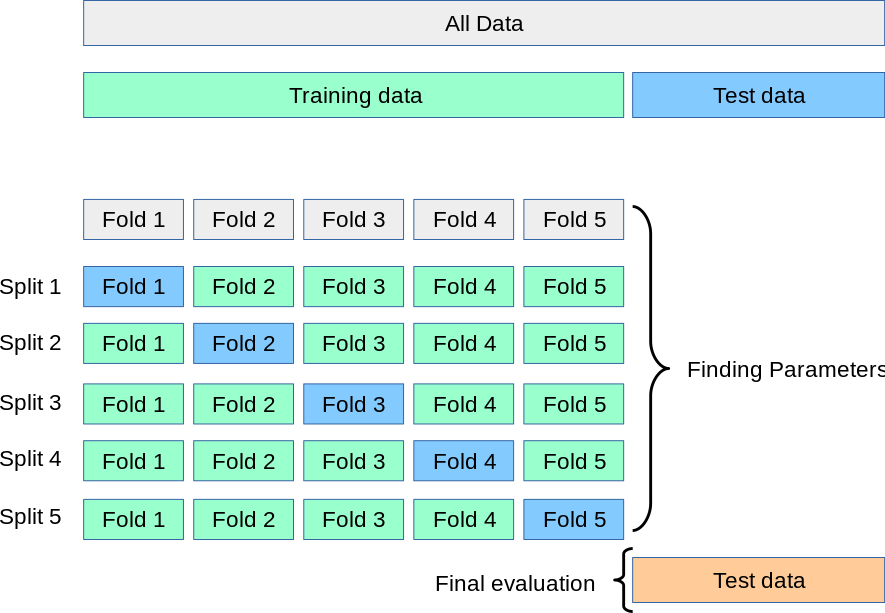
\includegraphics[scale=0.4]{grid_search_cross_validation.png}
	\caption{Ejemplo de validación cruzada con $k=5$}
	\label{fig:cross-validation}
\end{figure}
Como se aprecia en la figura \ref{fig:cross-validation}, se ha dividido el conjunto de datos en 5 conjuntos (folds), usando en cada iteración 4 para entrenar el modelo y uno para verificar con datos que el modelo no ha visto. Finalmente, se usa el conjunto de test (habiendo entrenado previamente el modelo con todo el conjunto de entrenamiento).
